\documentclass[letterpaper]{article}
\usepackage{natbib}
\usepackage[utf8]{inputenc}
\usepackage{graphicx}
\usepackage{color}
\usepackage{multirow}
\usepackage{amsmath}
\usepackage{array}
\usepackage{subcaption}
\usepackage{mathpazo}
\usepackage[a4paper]{geometry}
\usepackage{float}


\title{
\LARGE Learning Dynamics: Assignment 3 \\
\Large Multi-Armed Bandits and Stochastic Reward Game}
\author{\Large Hakim Boulahya \\ \\
hboulahy@ulb.ac.be - 000391737 \\ \\
\large Université Libre de Bruxelles \\
}

\begin{document}
\maketitle
\tableofcontents
\newpage

\section{N-Armed Bandit}

\paragraph{Remark} About the notation, the first arm/action starts
at \#0.

\subsection{Exercice 1}

\subsubsection{Average rewards}


% ex1 rewards
\begin{figure}[H]
    \centering
    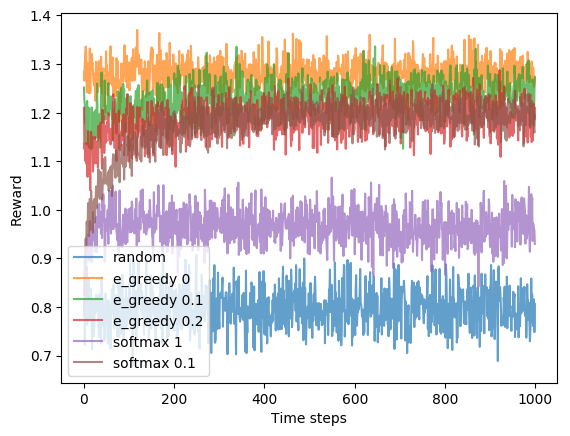
\includegraphics[width=.7\linewidth]{images/assign3/ex1/rewards}
    \caption{Average rewards for all algorithms}
    \label{fig:rewards_ex1}
\end{figure}

\paragraph{}

We can see that only exploring \textit{i.e.} random
and softmax with larger temperate $\tau = 1$ doesn't perform well, and
the reward stays low. Using softmax
with a temperature of 0.1 gives better results because
of the fact that it gets more greedy.

Using $\epsilon$-greedy with small
value, i.e. a large probability to choose the optimal actions,
tends
to better rewards. egreedy with 0 seems to arrives
\textit{directly} to the best arm. We can see on the graph that when $\epsilon$
is bigger it usually takes more time to get to the best arm, because of
the exploration.
Softmax with a temperature of 0.1 does tends to the best arm, but takes more
time.

\paragraph{}


It is important to note that the greedy behaviour is better, because
the standard deviation is small for this exercice. Because of that, using
the best action based on the estimated Q-values is accurate.

\subsubsection{Q-values estimation}

\label{sec:ex1_q_estim}

Figure \ref{fig:qtas_ex1} shows the estimation
of the Q-values for all algorithms.

% ex1 qtas
\begin{figure}[H]
  \begin{subfigure}{.5\textwidth}
    \centering
    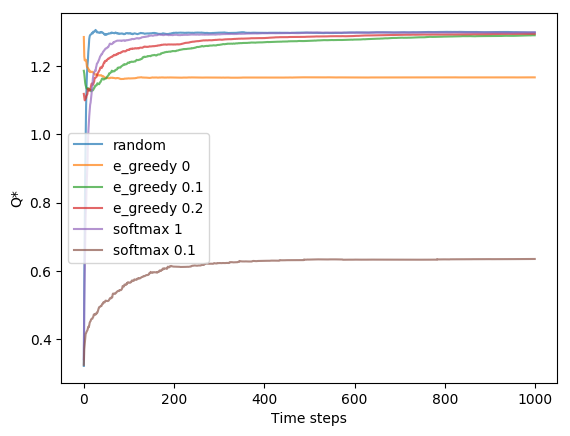
\includegraphics[width=1\linewidth]{images/assign3/ex1/qta_0}
    \caption{$Q_{a_{0}}(t)$}
    \label{fig:qta_0_ex1}
  \end{subfigure}
  \begin{subfigure}{.5\textwidth}
    \centering
    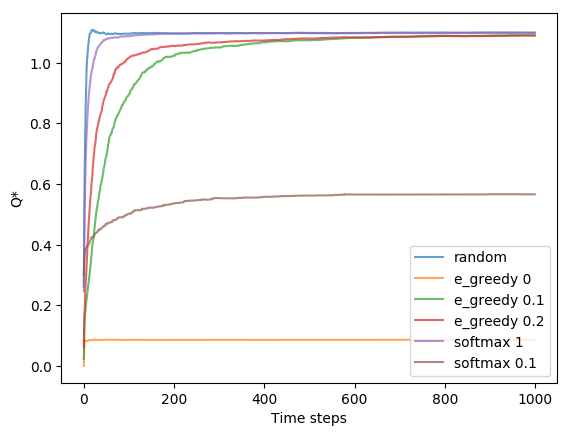
\includegraphics[width=1\linewidth]{images/assign3/ex1/qta_1}
    \caption{$Q_{a_{1}}(t)$}
    \label{fig:qta_1_ex1}
  \end{subfigure}
  \begin{subfigure}{.5\textwidth}
    \centering
    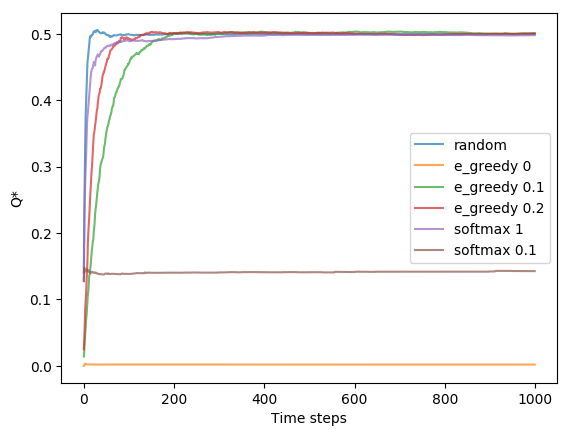
\includegraphics[width=1\linewidth]{images/assign3/ex1/qta_2}
    \caption{$Q_{a_{2}}(t)$}
    \label{fig:qta_2_ex1}
  \end{subfigure}
  \begin{subfigure}{.5\textwidth}
    \centering
    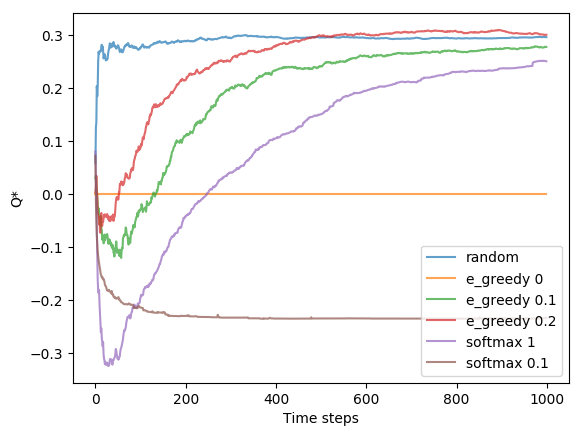
\includegraphics[width=1\linewidth]{images/assign3/ex1/qta_3}
    \caption{$Q_{a_{3}}(t)$}
    \label{fig:qta_3_ex1}
  \end{subfigure}

    \caption{Plot per arm showing
    the $Q^{*}_{a_{i}}$
    of that action along with the actual $Q_{a_{i}}$ a i estimate over time
    with
    $\mu$ = (1.3, 1.1, 0.5, 0.3), $\sigma$ = (0.9, 0.6, 0.4, 2.0)}
    \label{fig:qtas_ex1}
\end{figure}



\subsection*{Random}

Since random methods is full exploration, we can see that for all Q-values
the estimation of the $Q^*_{a_i}$ are accurate.


\subsection*{$\epsilon$-greedy}

\paragraph{$\epsilon = 0$} Using a \textit{only} greedy exploration, we
can see that only the best actions have Q-values different from 0. Actually
the best action \#0 tends to be estimated fast enough. For action \#1, the
Q-values is bigger than 0 because at the beginning of the learning, the
algorithm is still looking for the greedy action, therefore action \#1
could be the best one, until the algorithm find that \#action 0 is better.
The two other actions, are never explored since the it is a full greedy
method.

\paragraph{$\epsilon = \{0.1, 0.2\}$}

The estimation is more accurate when $\epsilon > 0$ \textit{i.e.} when
the action are also selected randomly which allows exploration. We can see
that by using a non-null $\epsilon$, the estimation of the Q-values overtime
tends to be accurate. An intersting observation is that the estimation
of the Q-values is faster (the accuration rate)
when $\epsilon$ is larger. This is logical,
since more $\epislon$ is large, more the action are selected randomly.

\subsection*{Softmax}

\paragraph{$\tau = 1$} Using $\tau = 1$ (a large enough temperature)
the Q-values estimation follows the same pattern as for any exploration methods
like random or $\epsilon = 0$. We can see that except for the last action
the curves are close to the random ones,
which confirm the exploration nature of a large temperature.
The fact that the curves of
the last action \#3 are more biased is because the standard deviation
is larger that for the other actions, which make the Q-values estimation
harder to make.


\paragraph{$\tau = 0.1$} Using a smaller temperature for the softmax
selection method, we have a more greedy action selection.
This action selection method is the worst one that estimate Q-values
(excluding the full exploiting method 0-greedy). We can see that
for the best arms \#0 and \#1, the estimations are larger than for there
worst arms, but it is \textit{far} from the actual $Q^*$. This can be explained
by the nature of the softmax selection method with a
small $\tau$: it sticks to the best arm
found and doesn't explore much to estimate the correct Q-values overtime.

\subsubsection{Histograms}

\label{sec:ex1_histo}

Figure \ref{fig:arms_ex1} shows the histograms for all algorithms.

% EX1 arms histograms
\begin{figure}[H]
  \begin{subfigure}{.5\textwidth}
    \centering
    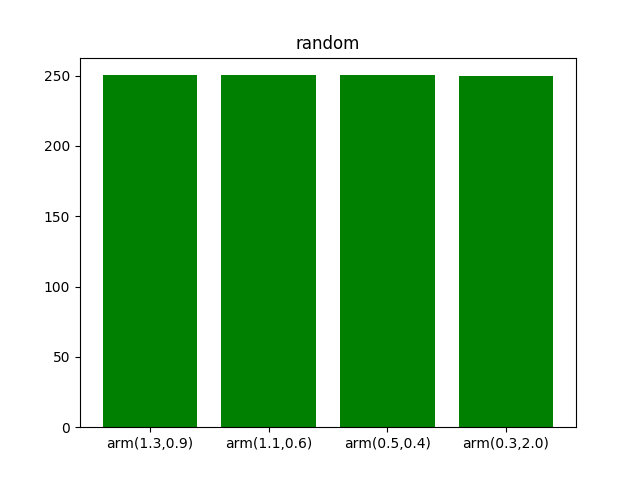
\includegraphics[width=1\linewidth]{images/assign3/ex1/arms_random}
    \caption{}
    \label{fig:arms_random_ex1}
  \end{subfigure}
  \begin{subfigure}{.5\textwidth}
    \centering
    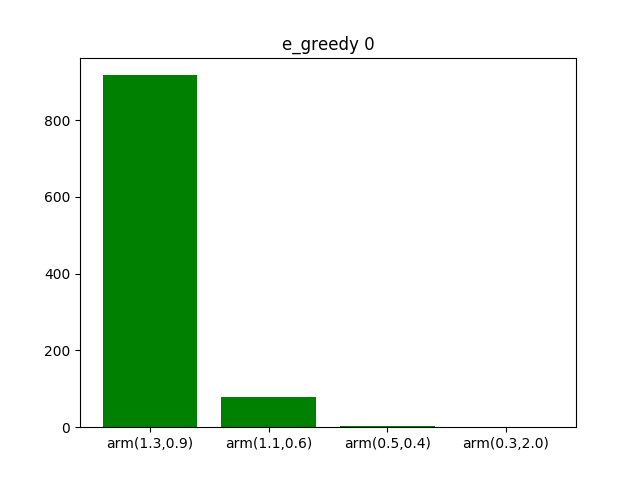
\includegraphics[width=1\linewidth]{images/assign3/ex1/arms_e_greedy0}
    \caption{}
    \label{fig:arms_e_greedy0_ex1}
  \end{subfigure}
  \begin{subfigure}{.5\textwidth}
    \centering
    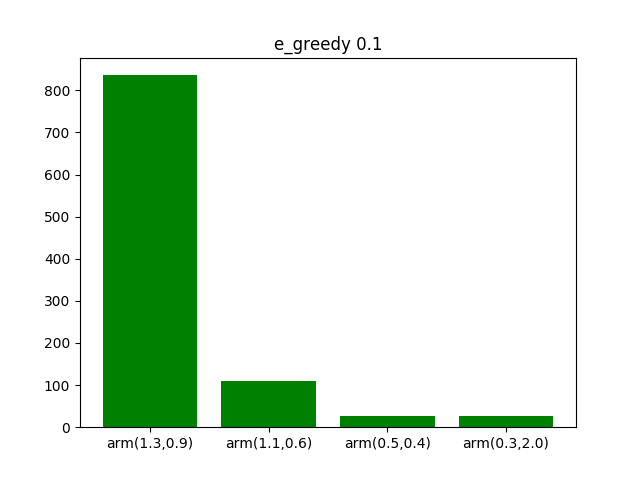
\includegraphics[width=1\linewidth]{images/assign3/ex1/arms_e_greedy01}
    \caption{}
    \label{fig:arms_e_greedy01_ex1}
  \end{subfigure}
  \begin{subfigure}{.5\textwidth}
    \centering
    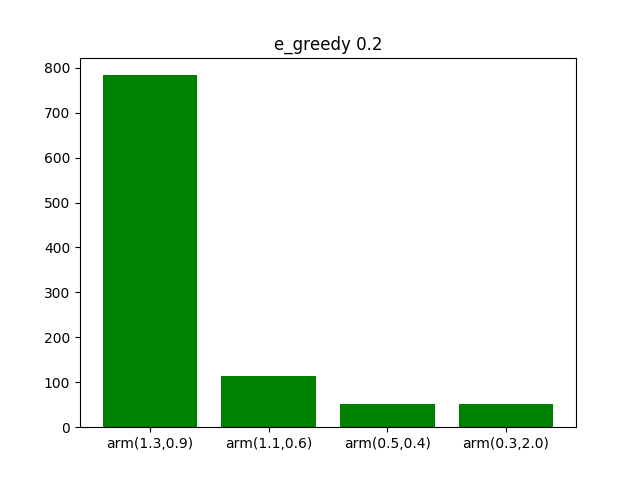
\includegraphics[width=1\linewidth]{images/assign3/ex1/arms_e_greedy02}
    \caption{}
    \label{fig:arms_e_greedy02_ex1}
  \end{subfigure}
  \begin{subfigure}{.5\textwidth}
    \centering
    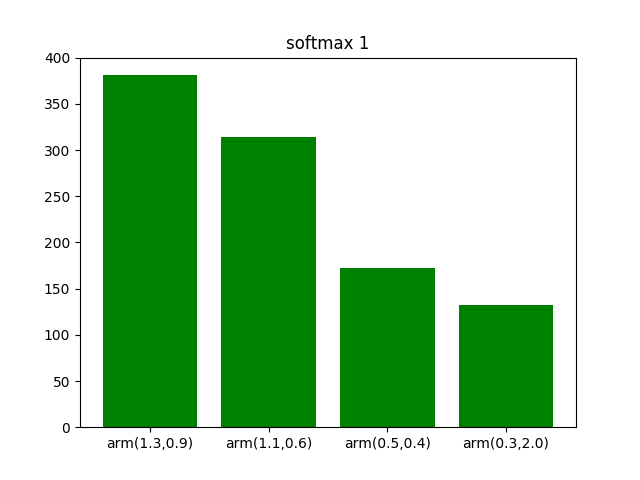
\includegraphics[width=1\linewidth]{images/assign3/ex1/arms_softmax1}
    \caption{}
    \label{fig:arms_softmax1_ex1}
  \end{subfigure}
  \begin{subfigure}{.5\textwidth}
    \centering
    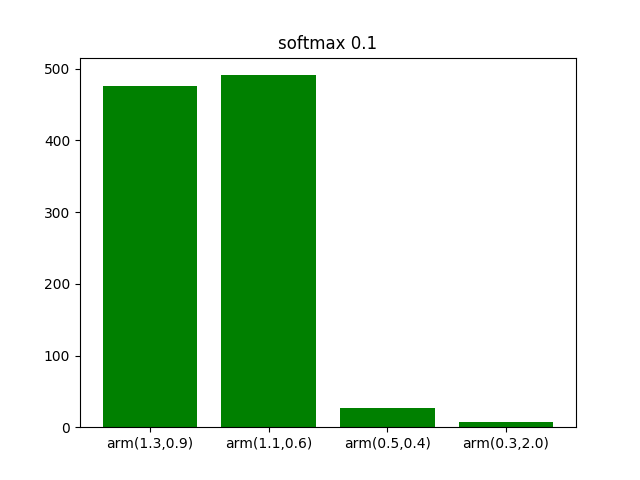
\includegraphics[width=1\linewidth]{images/assign3/ex1/arms_softmax01}
    \caption{}
    \label{fig:arms_softmax01_ex1}
  \end{subfigure}
    \caption{Histograms showing the number of times each action is selected
    per selection strategy with
    $\mu$ = (1.3, 1.1, 0.5, 0.3), $\sigma$ = (0.9, 0.6, 0.4, 2.0)}
    \label{fig:arms_ex1}
\end{figure}

\subsection*{Random}

\paragraph{}

The action selections, shown in Figure \ref{fig:arms_random_ex1},
for the random selection method is equidistributed.
Since all actions have the same probablity it is logical that the selection
is equidistributed when there $t \to \infty$.

\subsection*{$\epsilon$-greedy}


Figures \ref{fig:arms_e_greedy0_ex1}
\ref{fig:arms_e_greedy01_ex1}
\ref{fig:arms_e_greedy02_ex1} shows the histograms of action selections
for $\epsilon$-greedy selection methods.

\paragraph{$\epsilon = 0$}

With a null $\epsilon$, the action selection will be greedy \textit{i.e.},
and since we have a pretty small standard deviation, the best action \#0
is always chosen when found by the algorithm. This means that there is
no exploration, the method chooses the best arm directly. The fact that
the other actions are chosen, is that at the beginning it is necessary
to explore a little bit to find the best action.

\paragraph{$\epsilon = \{0.1, 0.2\}$}

It follows the same pattern that when $\epsilon$ is null, except that here
it is possible for the methods to explore more \textit{i.e.} choosing
other actions than the best one. This is why the bar of other actions
are higher when $\epsilon$ is bigger. If $\epsilon = 1$ the bars will
be as shown for the random methods in Figure \ref{fig:arms_random_ex1}.

\subsection*{Softmax}


Figures \ref{fig:arms_softmax1_ex1} \ref{fig:arms_softmax01_ex1}
shows the histograms of action selections
for softmax selection methods.

When temperature $\tau = 1$, the action selections are more randomize
\textit{i.e.} the exploration is more noticable. An interesting observation
in Figure \ref{fig:arms_softmax01_ex1}
is that when $\tau = 0.1$, \textit{i.e.}
the action selection is more greedy, softmax
algorithm tends to hesitate to choose the best actions. The
number of times that the 2 best actions,
action \#0 et \#1, are chosen is more or less equal.


\subsection{Exercice 2}

\subsubsection{Average rewards}

% ex2 rewards
\begin{figure}[H]
    \centering
    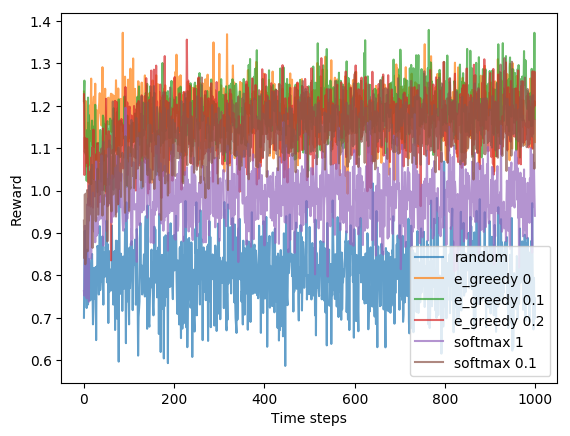
\includegraphics[width=.7\linewidth]{images/assign3/ex2/rewards}
    \caption{Average rewards for all algorithms}
    \label{fig:rewards_ex2}
\end{figure}

The results order of the algorithms that perform best doesn't really changes
compared to exercice 1.
By doubling the standard deviation, we only allowed the algorithms to
provide a more random rewards \textit{i.e.} a bigger range. We can see
that the dynamics of the algorithms don't change.

\paragraph{}

It is harder to learn because of the standard deviation that provides
a more randomize outcomes, therefore harder to find the best rewards.


\subsubsection{Q-values estimation}


Figure \ref{fig:qtas_ex2}
shows the estimation of the Q-values for all algorithms.

% ex2 qtas
\begin{figure}[H]
  \begin{subfigure}{.5\textwidth}
    \centering
    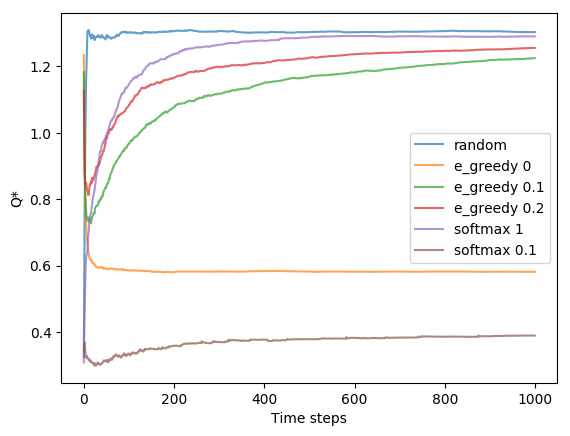
\includegraphics[width=1\linewidth]{images/assign3/ex2/qta_0}
    \caption{$Q_{a_{0}}(t)$}
    \label{fig:qta_0_ex2}
  \end{subfigure}
  \begin{subfigure}{.5\textwidth}
    \centering
    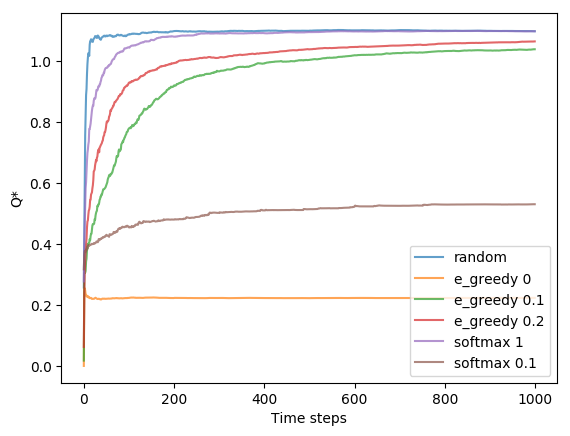
\includegraphics[width=1\linewidth]{images/assign3/ex2/qta_1}
    \caption{$Q_{a_{1}}(t)$}
    \label{fig:qta_1_ex2}
  \end{subfigure}
  \begin{subfigure}{.5\textwidth}
    \centering
    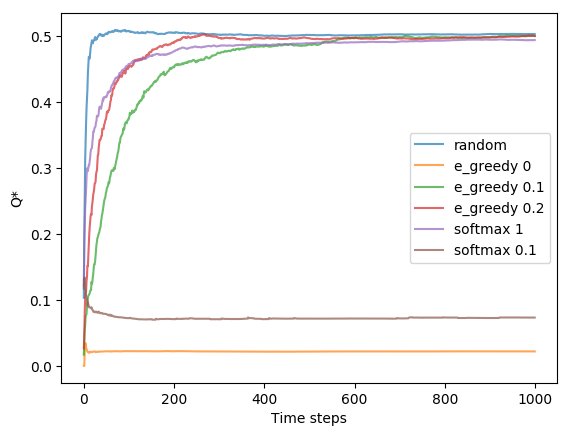
\includegraphics[width=1\linewidth]{images/assign3/ex2/qta_2}
    \caption{$Q_{a_{2}}(t)$}
    \label{fig:qta_2_ex2}
  \end{subfigure}
  \begin{subfigure}{.5\textwidth}
    \centering
    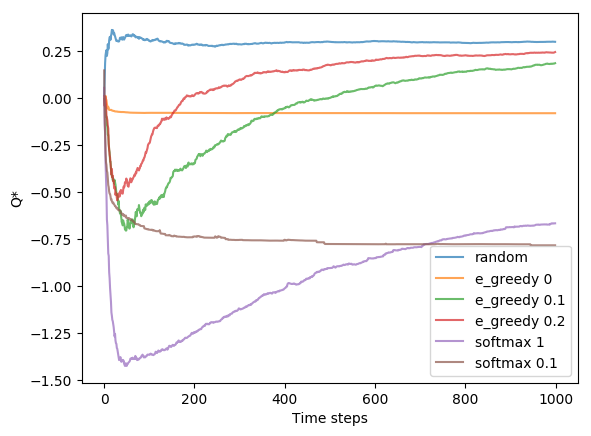
\includegraphics[width=1\linewidth]{images/assign3/ex2/qta_3}
    \caption{$Q_{a_{3}}(t)$}
    \label{fig:qta_3_ex2}
  \end{subfigure}

    \caption{Plot per arm showing
    the $Q^{*}_{a_{i}}$
    of that action along with the actual $Q_{a_{i}}$ a i estimate over time
    with
    $\mu$ = (1.3, 1.1, 0.5, 0.3), $\sigma$ = (1.8, 1.2, 0.8, 4.0)}
    \label{fig:qtas_ex2}
\end{figure}

\paragraph{}

The behaviour of the estimations for all algorithms are the same
that we explain in section \ref{sec:ex1_q_estim}. The major difference
is that the Q-values estimations for all algorithms, when exploring
takes more time, because the standard deviation is larger. Because of
that it is harder for the learner to estimate the correct Q-values.


\subsubsection{Histograms}


% ex2 arms histograms
\begin{figure}[H]
  \begin{subfigure}{.5\textwidth}
    \centering
    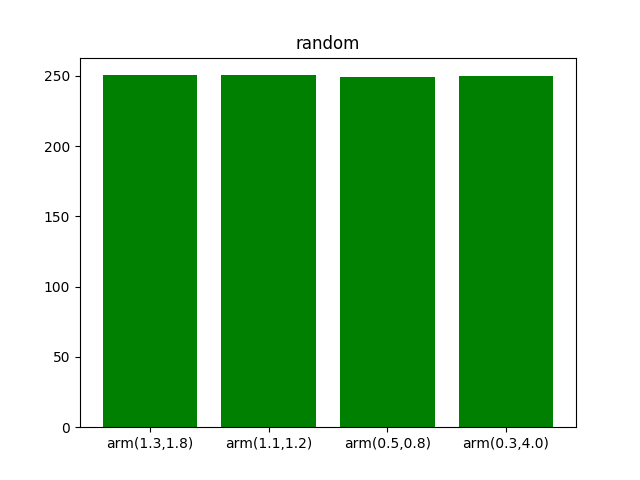
\includegraphics[width=1\linewidth]{images/assign3/ex2/arms_random}
    \caption{}
    \label{fig:arms_random_ex2}
  \end{subfigure}
  \begin{subfigure}{.5\textwidth}
    \centering
    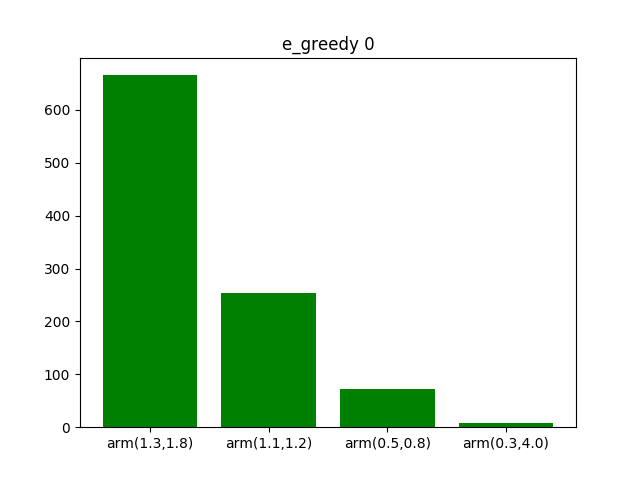
\includegraphics[width=1\linewidth]{images/assign3/ex2/arms_e_greedy0}
    \caption{}
    \label{fig:arms_e_greedy0_ex2}
  \end{subfigure}
  \begin{subfigure}{.5\textwidth}
    \centering
    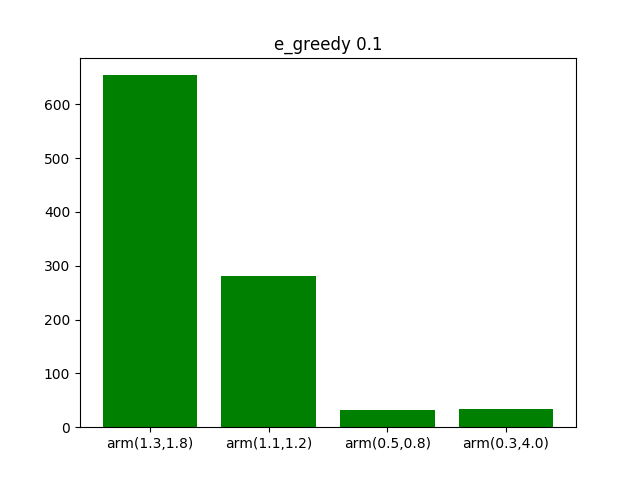
\includegraphics[width=1\linewidth]{images/assign3/ex2/arms_e_greedy01}
    \caption{}
    \label{fig:arms_e_greedy01_ex2}
  \end{subfigure}
  \begin{subfigure}{.5\textwidth}
    \centering
    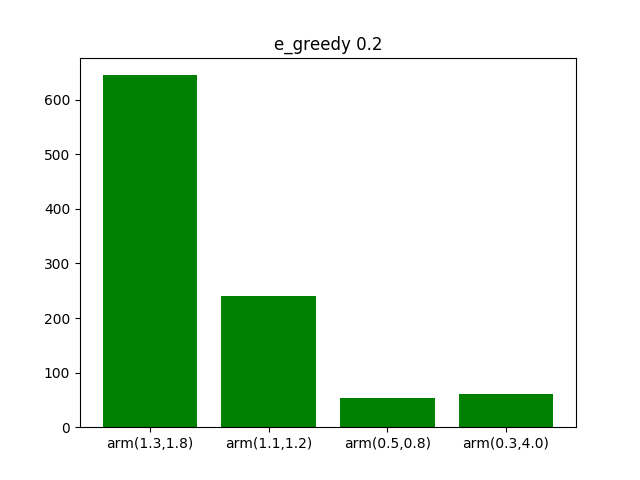
\includegraphics[width=1\linewidth]{images/assign3/ex2/arms_e_greedy02}
    \caption{}
    \label{fig:arms_e_greedy02_ex2}
  \end{subfigure}
  \begin{subfigure}{.5\textwidth}
    \centering
    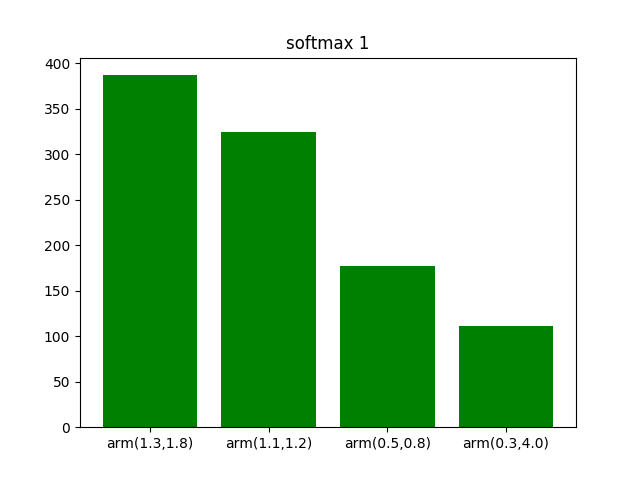
\includegraphics[width=1\linewidth]{images/assign3/ex2/arms_softmax1}
    \caption{}
    \label{fig:arms_softmax1_ex2}
  \end{subfigure}
  \begin{subfigure}{.5\textwidth}
    \centering
    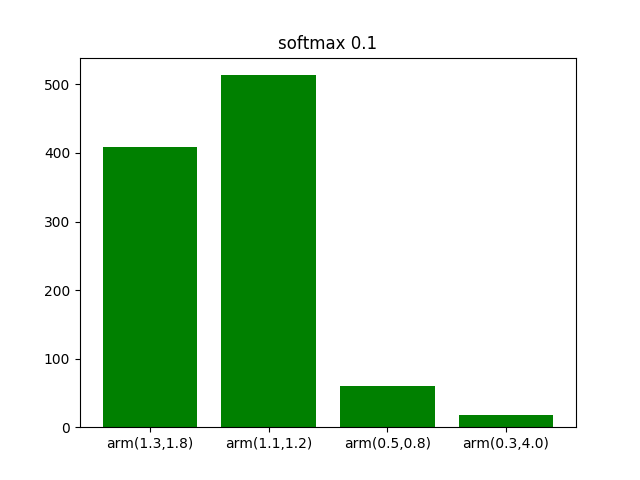
\includegraphics[width=1\linewidth]{images/assign3/ex2/arms_softmax01}
    \caption{}
    \label{fig:arms_softmax01_ex2}
  \end{subfigure}
    \caption{Histograms showing the number of times each action is selected
    per selection strategy with
    $\mu$ = (1.3, 1.1, 0.5, 0.3), $\sigma$ = (1.8, 1.2, 0.8, 4.0)}
    \label{fig:arms_ex2}
\end{figure}

\paragraph{}

The actions selection behaviour for all algorithms seems to follow
the same pattern that we explain in section \ref{sec:ex1_histo}.
The major difference is that for the one that exploit th most, for example
$0$-greedy, the selection of the \textit{worst} action have a higher
bars. This is because of the larger standard deviation for all actions.
It is harder to determine which one is the optimal selection \textit{i.e.}
the exploration at the beginning is necessary, because the Q-values
are estimated delayed compared to when the standard deviation is smaller.

\subsection{Exercice 3}

\subsubsection{Average rewards}

% ex3 rewards
\begin{figure}[H]
    \centering
    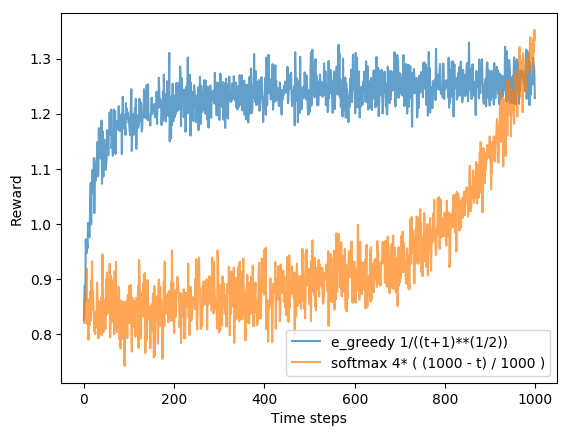
\includegraphics[width=.7\linewidth]{images/assign3/ex3/rewards}
    \caption{Average rewards for all algorithms}
    \label{fig:rewards_ex3}
\end{figure}

\paragraph{}

Dynamic $\epsilon$-greedy
doesn't seems to perform better that the static ones.
The resulting rewards tends to be identical. Observing the graph shows
that it takes more time to stabilize to the best arm.

\paragraph{}


Dynamic softmax seems to be better, if you consider the long term reward.
It takes to the 1000 epoch for the algorithm to find the best action reward in
opposition to the softmax using a a temperature of 0.1, where it
is close to the best arm at around epoch 200. But not as close as
the dynamic softmax, where it is closer to the best Q-value, when it
is stabilized.

\subsubsection{Q-values estimation}

\paragraph{}

Figure \ref{fig:qtas_ex3} shows the Q-values estimation overtime of
the dynamic selection methods $\epsilon$-greedy and softmax.

% ex3 qtas
\begin{figure}[H]
  \begin{subfigure}{.5\textwidth}
    \centering
    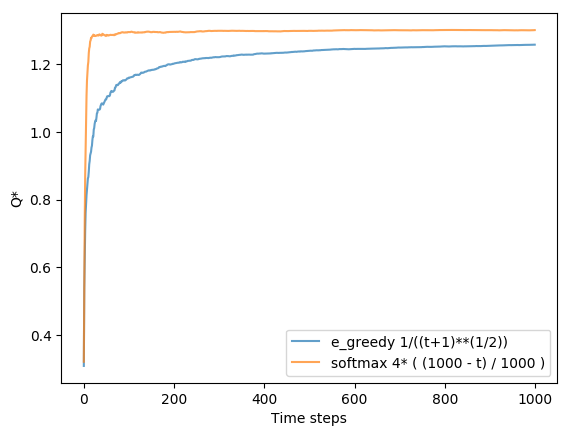
\includegraphics[width=1\linewidth]{images/assign3/ex3/qta_0}
    \caption{$Q_{a_{0}}(t)$}
    \label{fig:qta_0_ex3}
  \end{subfigure}
  \begin{subfigure}{.5\textwidth}
    \centering
    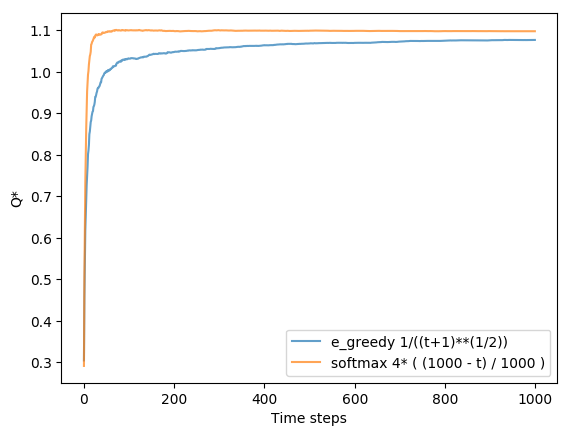
\includegraphics[width=1\linewidth]{images/assign3/ex3/qta_1}
    \caption{$Q_{a_{1}}(t)$}
    \label{fig:qta_1_ex3}
  \end{subfigure}
  \begin{subfigure}{.5\textwidth}
    \centering
    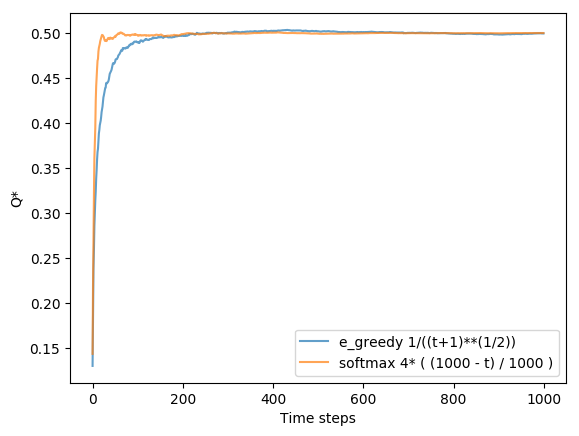
\includegraphics[width=1\linewidth]{images/assign3/ex3/qta_2}
    \caption{$Q_{a_{2}}(t)$}
    \label{fig:qta_2_ex3}
  \end{subfigure}
  \begin{subfigure}{.5\textwidth}
    \centering
    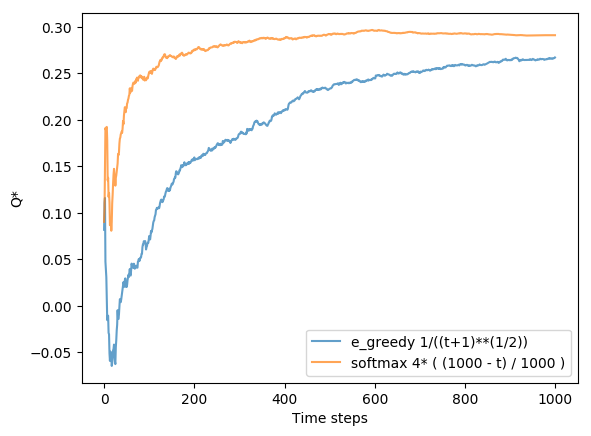
\includegraphics[width=1\linewidth]{images/assign3/ex3/qta_3}
    \caption{$Q_{a_{3}}(t)$}
    \label{fig:qta_3_ex3}
  \end{subfigure}

    \caption{Plot per arm showing
    the $Q^{*}_{a_{i}}$
    of that action along with the actual $Q_{a_{i}}$ a i estimate over time}
    \label{fig:qtas_ex3}
\end{figure}

\paragraph{Dynamic $\epsilon$-greedy}

Since the dynamic e-greedy method is randomize at the beginning and
more greedy overtime, the Q-values are correctly estimated and tends to
the correct $Q^*$ overtime.

\paragraph{Dynamic softmax}

We have a large temperature at the beginning and a smaller temperature overtime.
This leads to a algorithm that explore a lot at the beginning, therefore
estimate the Q-values very fast.

\subsubsection{Histograms}

% ex3 arms histograms
\begin{figure}[H]
    \begin{subfigure}{.5\textwidth}
    \centering
    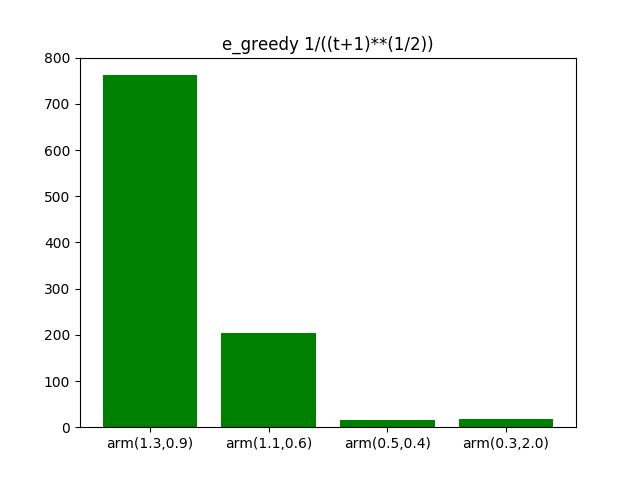
\includegraphics[width=1\linewidth]{images/assign3/ex3/arms_e_greedy_t}
    \caption{}
    \label{fig:arms_e_greedy_t_ex3}
    \end{subfigure}
    \begin{subfigure}{.5\textwidth}
      \centering
      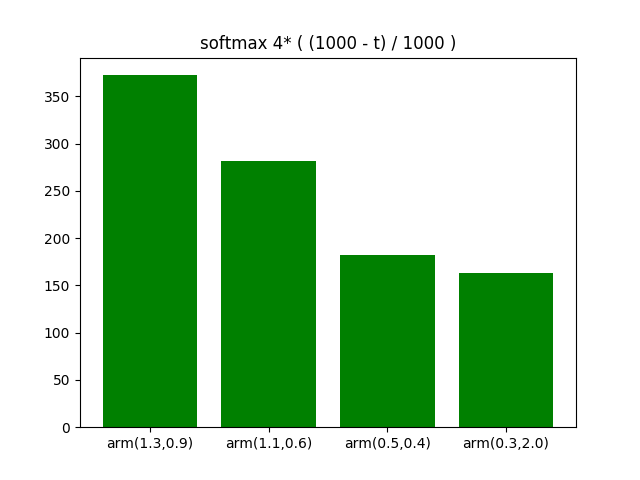
\includegraphics[width=1\linewidth]{images/assign3/ex3/arms_softmax_t}
      \caption{}
      \label{fig:arms_softmax_t_ex3}
    \end{subfigure}
    \caption{Histograms showing the number of times each action is selected
    per selection strategy}
    \label{fig:arms_ex3}
\end{figure}

\paragraph{Dynamic $\epsilon$-greedy}

The action selection tends to the optimal action \#0 very fast. This
is because that the probability $\epsilon$ drops very fast overtime, which
lead to the greedy selection behaviour.

\paragraph{Dynamic softmax}

Since dynamic softmax has a large temperature when $t$ is small, therefore
explore a lot, we can see that all actions are selected. Overtime
to selection will be more greedy, and since the Q-values are accurate
because of the exploration, when $t$ is high enough, the action \#0 and \#1
will be selected more often. That explains the \textit{stairs} form
of the histogram.

\section{Climbing game}

When using the formula, it is important to have a big tau, because exp(Q/tau)
will give errors if Q is too big. (See how EV(a) is calculated)

I also remarked that when using EV with max_rewards or max_q when
min_tau = 0.001 the 11 is good, but when 0.1 or 1, not. THis is probably
due to the stochastic of our game.

\end{document}
